\subsection{General Object Recognition}
To analyze the ability of the deep features to transfer to basic-level object category recognition, we evaluate them on the Caltech-101 dataset~\cite{caltech101}.
In addition to directly evaluating linear classifier performance on FC$_6$ and FC$_7$, we also report results using the dropout regularization technique proposed by~\cite{hintondropout}, which is also present in the Imagenet training phase.
At training time, this technique works by randomly setting half of the activations (here, our features) in a given layer to 0.
At test time, all activations are multiplied by 0.5.
Dropout was used successfully by~\cite{supervision} in layers 6 and 7 of their network; hence we study the effect of the technique when applied to the features derived from these layers.

In each evaluation, the classifier, a logistic regression (LogReg) or support vector machine (SVM), is trained on a random set of 30 samples per class (including the background class), and tested on the rest of the data, with parameters cross-validated for each split on a 25 train/5 validation subsplit of the training data.
The results in Table \ref{tab:caltech101results} are reported in terms of mean accuracy per category averaged over five data splits.

\begin{table}
\centering
\begin{tabular}{lccc}
\hline
& POOL$_5$ & FC$_6$ & FC$_7$ \\
\hline
LogReg & $63.29 \pm 6.6$ & $84.30 \pm 1.6$ & $84.87 \pm 0.6$ \\
LogReg with Dropout & - & $86.08 \pm 0.8$ & $85.68 \pm 0.6$ \\
SVM & $77.12 \pm 1.1$ & $84.77 \pm 1.2$ & $83.24 \pm 1.2$ \\
SVM with Dropout & - & $\mathbf{86.91 \pm 0.7}$ & $85.51 \pm 0.9$ \\
\hline
Yang \etal\cite{yang09} & \multicolumn{3}{c}{84.3} \\
Jarrett \etal\cite{jarrett09} & \multicolumn{3}{c}{65.5} \\
\hline
\end{tabular}
\caption{Average accuracy per class on Caltech-101 with 30 training samples per class across three hidden layers of the network and two classifiers.
Our result from the training protocol/classifier combination with the best validation accuracy -- SVM with Layer 6 (+ dropout) features -- is shown in \textbf{bold}.}\label{tab:caltech101results}
\end{table}

\begin{figure}
  \centering
  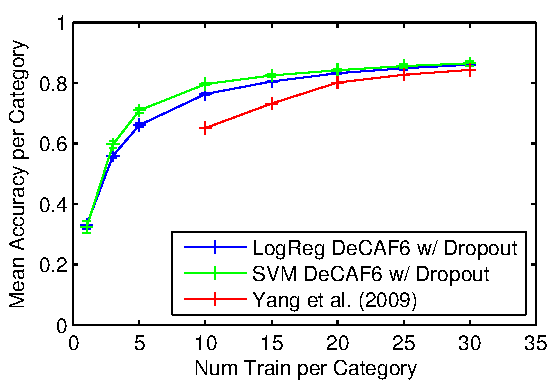
\includegraphics[width=0.5\textwidth]{figs/decaf/caltech101_plot_numtrain.pdf}
  \caption{Average accuracy per class on Caltech-101 at varying training set sizes.}\label{fig:caltech101results}
\end{figure}

Our top-performing method (based on validation accuracy) trains a linear SVM on FC$_6$ with dropout, with test set accuracy of 86.9\%.
The POOL$_5$ features perform substantially worse than either the FC$_6$ or FC$_7$ features, and hence we do not evaluate them further in this paper.
The FC$_7$ features generally have accuracy about 1-2\% lower than the FC$_6$ features on this task.
The dropout regularization technique uniformly improved results by 0-2\% for each classifier/feature combination.
When trained on the deep features, the SVM and logistic regression classifiers perform roughly equally well on this task.

We compare our performance against the current state-of-the-art on this benchmark from~\cite{yang09}, a method employing a combination of 5 traditional hand-engineered image features followed by a multi-kernel based classifier.
Our top-performing method outperforms this method by 2.6\%. Note that it is likely that our features could be added to the set of hand-engineered features inside of the method of~\cite{yang09} to achieve even higher performance, but we focus here only on very simple, fast methods to demonstrate the representational strength of the features alone.
Our method also outperforms by over 20\% the two-layer convolutional network of~\cite{jarrett09}, demonstrating the importance of the depth of the network used for our feature.
Note that unlike our method, these approaches from the literature do not implicitly leverage an outside large-scale image database like ImageNet.
The performance edge of our method over these approaches demonstrates the importance of multi-task learning when performing object recognition with sparse data like that available in the Caltech-101 benchmark.

To further explore the impact of sparse training data on our method's performance, we also show how performance of the two Layer 6 + dropout methods above vary with the number of training cases per category, plotted in Figure~\ref{fig:caltech101results}. Results are again given in terms of mean accuracy per class averaged across five random data splits, and parameters in this case were kept fixed. The $i^{\mathrm{th}}$training set split at size $M$ is a subset of the $i^{\mathrm{th}}$ split at size $N$ for any $N > M$ to ensure consistency between results. Surprisingly, with just a \textit{single} labeled instance per category (one-shot learning) we are able to learn a reasonably useful classifier on the 102-category classification task, achieving accuracy of 33.0\% compared to chance accuracy of $<1$\%. This suggest that with sufficiently strong representations like the ones in this thesis, useful models of visual categories can often be learned from just a single positive example.

\subsection{Domain Adaptation}
We next evaluate the deep features for use on the task of domain adaptation. For our experiments we use the benchmark \textit{Office} dataset \cite{eccv_saenko}.The dataset contains three domains: \texttt{Amazon}, which consists of product images taken from \url{amazon.com}; and \texttt{Webcam} and \texttt{Dslr}, which consist of images taken in an office environment using a webcam or digital SLR camera, respectively. 

In the domain adaptation setting, we are given a training (source) domain with labeled training data and a distinct test (target) domain with either a small amount of labeled data or no labeled data. We will experiment within the supervised domain adaptation setting, where there is a small amount of labeled data available from the target domain. 

Most prior work for this dataset uses SURF \cite{surf06} interest point features (available for download with the dataset). To illustrate the ability of DeCAF to be robust to resolution changes, we use the t-SNE~\cite{tsne} algorithm to project both SURF and FC$_6$, computed for \texttt{Webcam} and \texttt{Dslr}, into a 2D visualizable space (See Figure~\ref{fig:office_vis}). We visualize an image on the point in space corresponding to its low dimension projected feature vector. We find that the deep features not only provides better within category clustering, but also clusters same category instances across domains, effectively \emph{undoing} the domain bias, or the ``dataset bias'' as described by Torralba and Efros \cite{torralba2011unbiased}.

\newcommand{\soffice}{.3\linewidth}
\begin{figure}
\centering
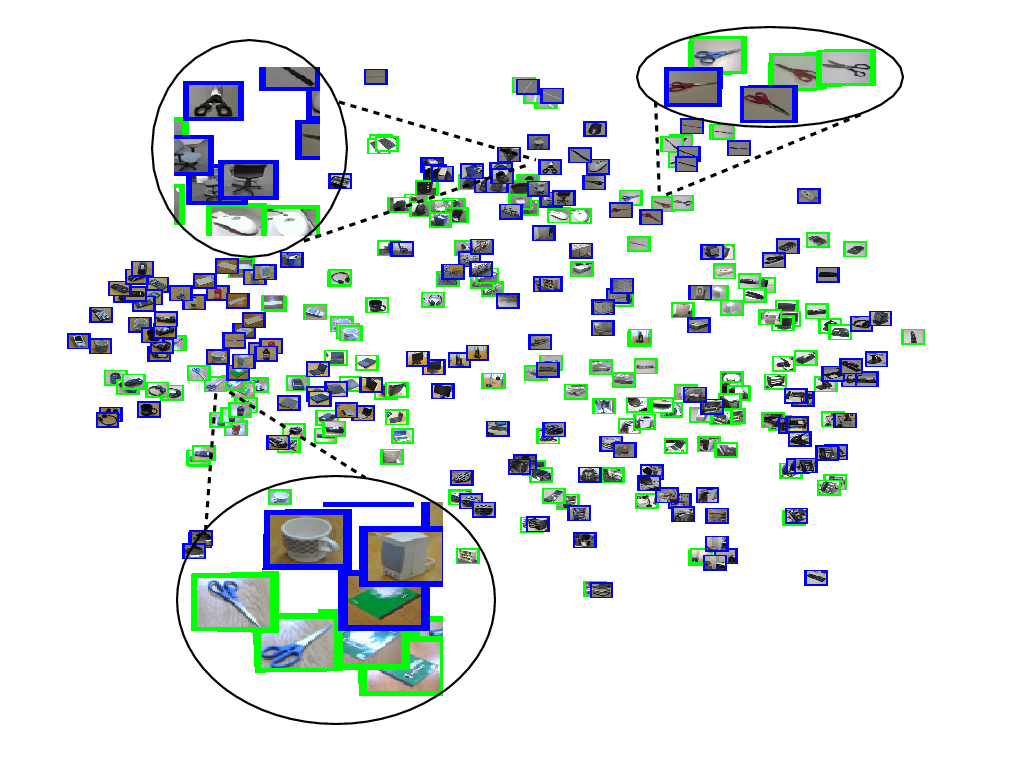
\includegraphics[height=\soffice]{figs/decaf/surf_webcam_dslr_vis_overlay.png}
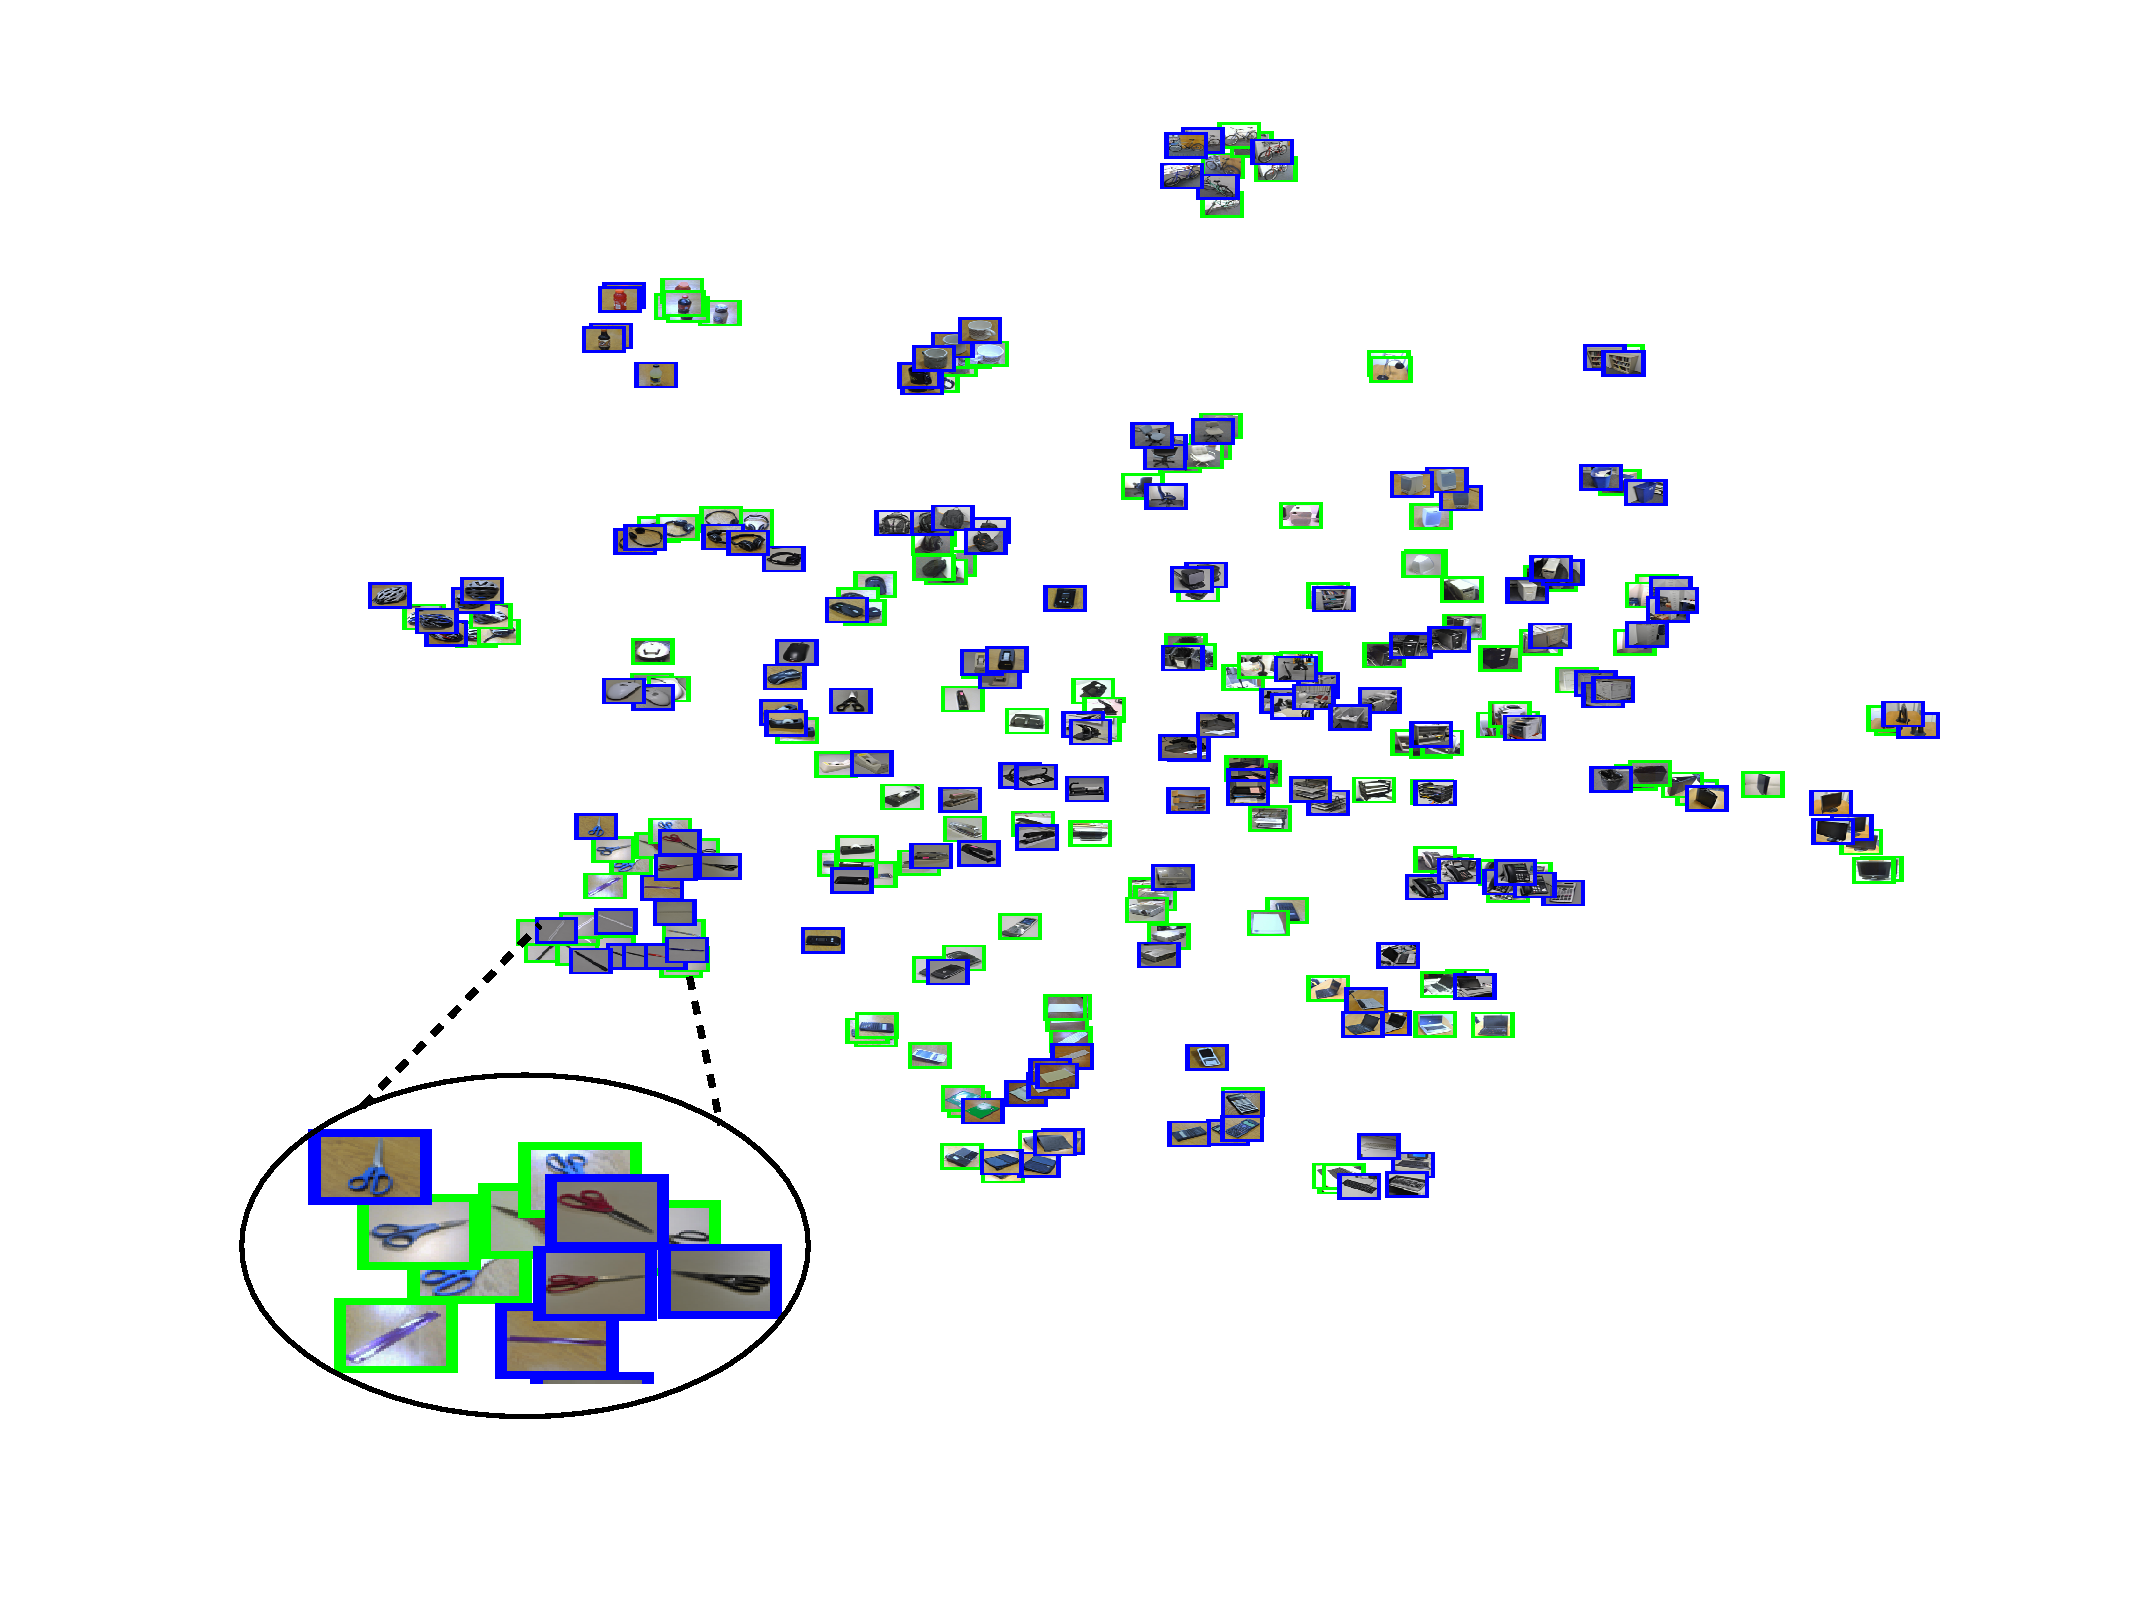
\includegraphics[height=\soffice]{figs/decaf/fc6_webcam_dslr_vis_overlay1}
\caption{Visualization of the webcam (green) and dslr (blue) domains using the original released SURF features (left) and FC$_6$ (right). The figure is best viewed by zooming in to see the images in local regions. All images from the scissor class are shown enlarged. They are well clustered and overlapping in both domains with our representation, while SURF only clusters a subset and places the others in disjoint parts of the space, closest to distinctly different categories such as chairs and mugs.}
\label{fig:office_vis}
\end{figure}

\newcommand{\ra}[1]{\renewcommand{\arraystretch}{#1}}

\begin{table}
\small
\begin{center}
\ra{1.1}
\tabcolsep=0.11cm
\begin{tabular}{@{} cccccccc @{}}
& \multicolumn{3}{c}{\texttt{Amazon} $\rightarrow$ \texttt{Webcam}} & \phantom{ab} & \multicolumn{3}{c}{\texttt{Dslr} $\rightarrow$ \texttt{Webcam}}\\
\cmidrule{2-4} \cmidrule{6-8}
	& SURF & FC$_6$ & FC$_7$  && SURF& FC$_6$ & FC$_7$\\
        	\midrule
LogReg(S) & $  9.63\pm    1.4$ & $ 48.58\pm    1.3$ & $ 53.56\pm    1.5$ && $ 24.22\pm    1.8 $ & $ 88.77\pm    1.2$ & $ 87.38\pm    2.2$ \\
SVM(S) & $ 11.05\pm    2.3$ & $ 52.22\pm    1.7$ & $ 53.90\pm    2.2$ && $ 38.80\pm    0.7 $ & $ 91.48\pm    1.5$ & $ 89.15\pm    1.7$ \\
%\\
LogReg(T) & $ 24.33\pm    2.1$ & $ 72.56\pm    2.1$ & $ 74.19\pm    2.8$ && $ 24.33\pm    2.1 $& $ 72.56\pm    2.1$ & $ 74.19\pm    2.8$ \\
SVM(T) & $ 51.05\pm    2.0$ &  $ 78.26\pm    2.6$ & $ 78.72\pm    2.3$ && $ 51.05\pm    2.0 $&  $ 78.26\pm    2.6$ & $ 78.72\pm    2.3$ \\
%\\
LogReg(ST) & $ 19.89\pm    1.7$  & $ 75.30\pm    2.0$ & $ 76.32\pm    2.0$ && $ 36.55\pm    2.2 $ & $ 92.88\pm    0.6$ & $ 91.91\pm    2.0$ \\
SVM(ST) & $ 23.19\pm    3.5$  & $ 80.66\pm    2.3$ & $ 79.12\pm    2.1$ && $ 46.32\pm    1.1 $&$\bm{ 94.79\pm    1.2}$ & $ 92.96\pm    2.0$ \\
 \\
\cite{ref:daume} & $ 40.26\pm    1.1$  & $\bm{82.14\pm    1.9}$ & $ 81.65\pm    2.4$ && $ 55.07\pm    3.0 $ & $ 91.25\pm    1.1$ & $ 89.52\pm    2.2$ \\
\cite{Hoffman13:ELD} & $ 37.66\pm    2.2$  & $ 80.06\pm    2.7$ & $ 80.37\pm    2.0$ && $ 53.65\pm    3.3 $ & $ 93.25\pm    1.5$ & $ 91.45\pm    1.5$ \\
\cite{ref:gong12_gfk} & $ 39.80\pm    2.3$ &  $ 75.21\pm    1.2$ & $ 77.55\pm    1.9$ & &$ 39.12\pm    1.3 $ & $ 88.40\pm    1.0$ & $ 88.66\pm    1.9$ \\
\cite{ref:dlid} & \multicolumn{3}{c}{58.85} && \multicolumn{3}{c} {78.21}\\
\hline
\end{tabular} 
\end{center}
\caption{Deep features dramatically outperforms the baseline SURF feature available with the \textit{Office} dataset as well as the deep adaptive method of \cite{ref:dlid}. We report average multi-class accuracy using both standard and adaptive classifiers, changing only the input feature from SURF to deep features. Surprisingly, in the case of \texttt{Dslr}$\rightarrow$\texttt{Webcam} the domain shift is largely non-existent with the new features.}
\label{tab:office}
\end{table}

We validate this conclusion with a quantitative experiment on the \textit{Office} dataset. Table \ref{tab:office} presents multi-class accuracy averaged across 5 train/test splits for the domain shifts \texttt{Amazon}$\rightarrow$\texttt{Webcam} and \texttt{Dslr} $\rightarrow$ \texttt{Webcam}. We use the standard experimental setup first presented in \cite{eccv_saenko}. To compare SURF with the FC$_6$ and FC$_7$ features, we report the multi-class accuracy for each, using an SVM and Logistic Regression both trained in 3 ways: with only source data (S), only target data (T), and source and target data (ST). We also report results for three adaptive methods run with each deep feature we consider as input. Finally, for completeness we report a recent and competing deep domain adaptation result from \cite{ref:dlid}. It is observed that by adopting deep features alone, one could dramatically outperform the baseline SURF feature available with the \textit{Office} dataset as well as the deep adaptive method of \cite{ref:dlid}. 


\begin{figure}[t]
\centering
\begin{tabular}{ccc}
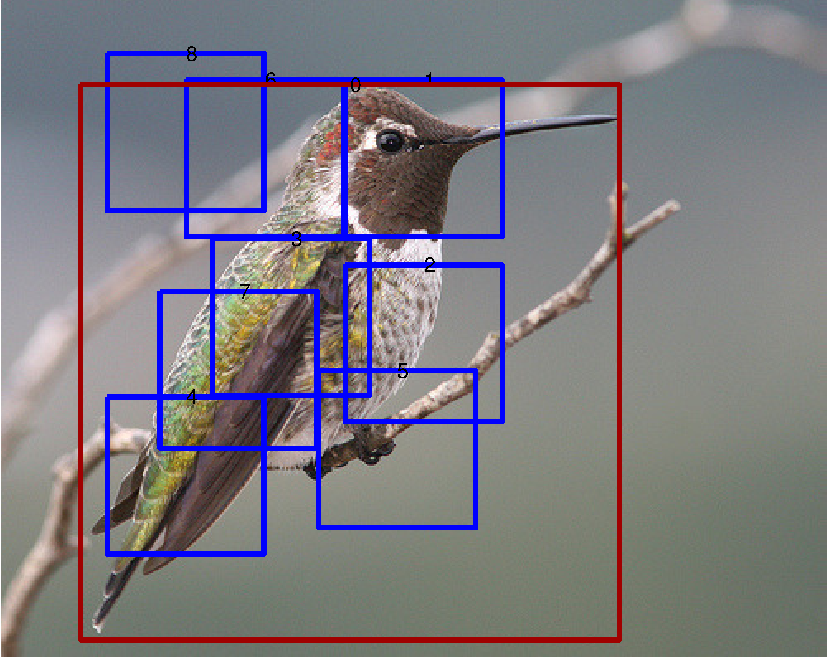
\includegraphics[height=0.3\linewidth]{figs/decaf/bird_detection} &
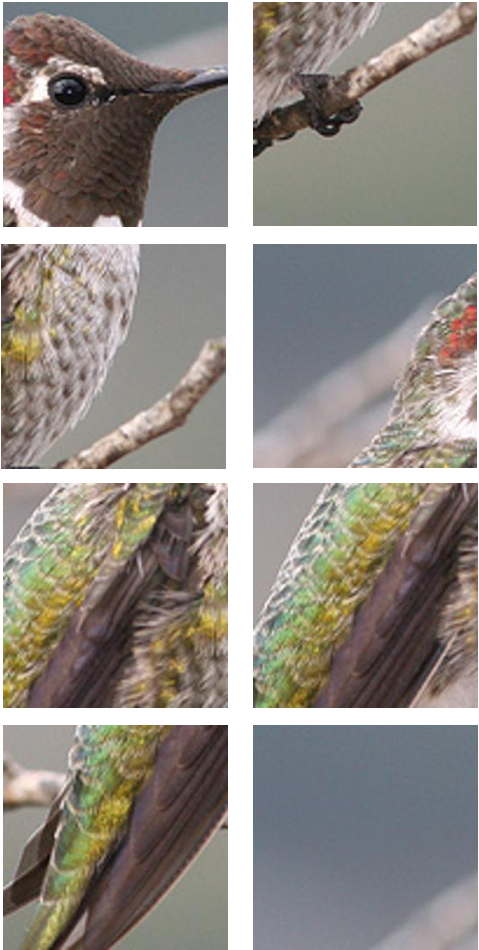
\includegraphics[height=0.3\linewidth]{figs/decaf/bird_with_parts} &
\raisebox{24mm}{\begin{minipage}{.2\linewidth}
\centering
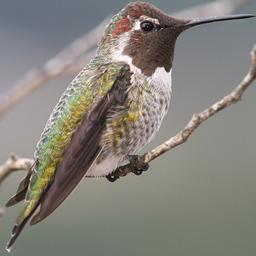
\includegraphics[height=0.47\linewidth]{figs/decaf/bbox.jpg} \\
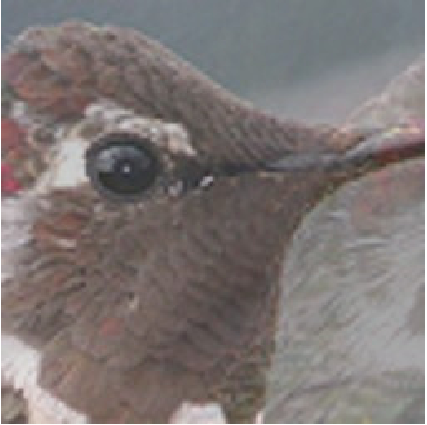
\includegraphics[height=0.47\linewidth]{figs/decaf/bird_head} \\
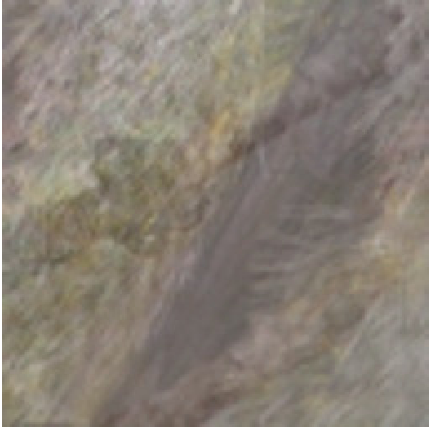
\includegraphics[height=0.47\linewidth]{figs/decaf/bird_body}
\end{minipage}}\\
DPM Detections & Parts & DPD \\
\end{tabular}
\caption{The pipeline of the deformable part descriptor (DPD) on a sample test images. It uses DPM for part localization and then uses learned pooling weights for the final pose-normalized representation.}
\label{fig:birds}
\end{figure}

\begin{table}
\centering
\begin{tabular}{lc}
\toprule
Method & Accuracy\\
\midrule
FC$_6$  & 58.75 \\
DPD + FC$_6$ & {\bfseries 64.96} \\
\\
DPD \cite{dpd}& 50.98 \\
POOF \cite{poof}& 56.78 \\
\bottomrule
\end{tabular}
\caption{Accuracy on the Caltech-UCSD bird dataset.}
\label{table:birds}
\end{table}

\subsection{Fine-Grained Recognition}
We tested the performance of deep features on the task of subcategory recognition. To this end, we adopted one of its most popular tasks - the Caltech-UCSD birds dataset~\cite{birds}, and compare the performance against several state-of-the-art baselines.

Following common practice in the literature, we adopted two approaches to perform classification. Our first approach adopts an ImageNet-like pipeline, in which we followed the existing protocol by cropping the images regions $1.5\times$ the size of the provided bounding boxes, resizing them 256$\times$256 and then feeding them into the convolutional pipeline to get the features for classification. For simplicity, we computed FC$_6$ and trained a multi-class logistic regression on top of the features.

Our second approach, we tested the deep features in a pose-normalized setting using the deformable part descriptors (DPD) method~\cite{dpd}. Inspired by the deformable parts model \cite{dpm}, DPD explicitly utilizes the part localization to do semantic pooling. Specifically, after training a weakly-supervised DPM on bird images, the pool weight for each part of each component is calculated by using the key-point annotations to get cross-component semantic part correspondence. The final pose-normalized representation is computed by pooling the image features of predicted part boxes using the pooling weights. Based on the DPD implementation provided by the authors, we applied deep feature extraction in the same pre-trained DPM model and part predictions and used the same pooling weights. Figure \ref{fig:birds} shows the DPM detections and visualization of pooled DPD features on a sample test image.  As our first approach, we resized each predicted part box to 256 $\times$ 256 and computed FC$_6$ to replace the KDES image features \cite{kdes} used in DPD paper.

Our performance as well as those from the literature are listed in Table \ref{table:birds}. Deep features together with a simple logistic regression already obtains a significant performance increase over existing approaches, indicating that such features, although not specifically designed to model subcategory-level differences, captures such information well. In addition, explicitly taking more structured information such as part locations still helps, and provides another significant performance increase, obtaining an accuracy of 64.96\%, compared to the 50.98\% accuracy reported in~\cite{dpd}. It also outperforms POOF \cite{poof}, to our knowledge the best accuracy reported in the literature prior to this work.

We note again that in all the experiments above, no fine-tuning is carried out on the lower-level layers, since our main interest is to analyze how well a feature extraction pipeline trained with a different objective generalizes to different tasks. To obtain the best possible result one may want to perform a full back-propagation, as have been shown effective in specific applications like detection \cite{girshick2013rich}. However, the fact
that we see a significant performance increase without fine-tuning suggests that
a pretrained deep network may already serve as a good off-the-shelf visual representation without heavy computation.

\subsection{Scene Recognition}
Finally, we evaluate DeCAF on the scene recognition benchmarks, namely the SUN-397 large-scale scene recognition database~\cite{xiao10}. Unlike object recognition, wherein the goal is to identify and classify an object which is usually the primary focus of the image, the goal of a scene recognition task is to classify the \textit{scene} of the entire image.
In the SUN-397 database, there are 397 semantic scene categories including \textit{abbey}, \textit{diner}, \textit{mosque}, and \textit{stadium}.
Because DeCAF is learned on ILSVRC, an object recognition database, we are applying it to a task for which it was not designed.
Hence we might expect this task to be very challenging for these features, unless they are highly generic representations of the visual world.

Based on the success of using dropout with FC$_6$ and FC$_7$ for the object recognition task detailed in Section~\ref{sec:caltech}, we train and evaluate linear classifiers on these dropped-out features on the SUN-397 database.
Table~\ref{tab:sunresults} gives the classification accuracy results averaged across 5 splits of 50 training images and 50 test images.
Parameters are fixed for all methods, but we select the top-performing method by cross-validation, training on 42 images and testing on the remaining 8 in each split.

Our top-performing method in terms of cross-validation accuracy was to use FC$_7$ with the SVM classifier, resulting in 40.94\% test performance.
Comparing against the method of~\cite{xiao10}, the current state-of-the-art method, we see a performance improvement of 2.9\% using the feature off-the-shelf and without any ensembles with additional features.
Note that, like the state-of-the-art method used as a baseline in Section~\ref{sec:caltech}, this method uses a large set of traditional vision features and combines them with a multi-kernel learning method.
The fact that a simple linear classifier on top of our single image feature outperforms the multi-kernel learning baseline built on top of many traditional features demonstrates the ability of DeCAF to generalize to other tasks and its representational power as compared to traditional hand-engineered features.

\begin{table}
\centering
\begin{tabular}{lcc}%{|c|c|c|}
\hline
& FC$_6$ & FC$_7$ \\
\hline
LogReg & $\bm{ 40.94 \pm 0.3}$ & $40.84 \pm 0.3$ \\
SVM & $39.36 \pm 0.3$ & $40.66 \pm 0.3$ \\
\hline
Xiao \etal \cite{xiao10} & \multicolumn{2}{c}{38.0} \\
\hline
\end{tabular}
\caption{Average accuracy per class on SUN-397 with 50 training samples and 50 test samples per class, across two hidden layers of the network and two classifiers. Note that the result from the training protocol/classifier combination with the best validation accuracy is FC$_7$, while FC$_6$ has the best testing accuracy. However the difference between them is not statistically significant.}
\label{tab:sunresults}
\end{table}